\chapter{Resin injection bolted joint with reload}
\label{app3}
\onehalfspacing

\section{Introduction for Resin injection bolt}

 High-strength bolts (hereinafter HSB) are extensively employed worldwide as friction-type bolted connections (referred to as friction connections) for joining steel members. Bolted connections play a crucial role in steel structures, as the inadequate performance of a weak connection can lead to the loss of structural integrity and stability. However, in many cases, there may be instances of insufficient slip resistance, for example, when the slip coefficient of the mating surface cannot be guaranteed or when enlarged holes are used. Therefore, it is crucial to propose a connection method that improves slip resistance by building upon existing friction connections to meet the requirements of the design.

\begin{figure}[htbp]
    \centering
    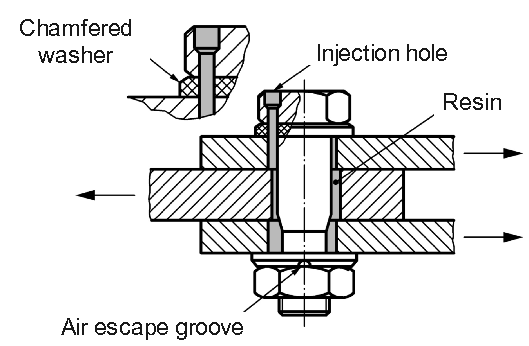
\includegraphics[width=0.75\linewidth]{imgs//app3/iR-mecha.pdf}
    \caption{Resin injection bolt in a double shear connection according to EN 1090-2, Annex J}
    \label{fig-RI-mecha}
\end{figure}
    
 Resin-injected bolts are fasteners that utilise a two-component resin to fill the clearance between the bolt and the hole wall, as depicted in Fig. \ref{fig-RI-mecha}. They serve as an effective alternative to fit bolts when high bolt hole accuracy is required, or the oversized hole was used. Injection bolts offer a reliable, cost-effective solution for repairing and enhancing existing structures \cite{gresnigt1996injbolt}. Moreover, they have proven successful in the construction of new structures. The clearance of an injection bolt is filled through a small hole in its head. Once the resin injection is complete and fully cured, the connection becomes resistant to slip. The bolt's bearing and shear resistance is used to transfer the external load, see  Fig. 1. Additionally, standard structural bolts can be adapted for use as injection bolts. These bolts and washers undergo modifications to facilitate resin injection. The design and execution guidelines for injection bolts are established by the recommendations of ECCS \cite{eccs1985} and Eurocode3 \cite{eurocode3-21,en1090-2-2018} for steel structures.
 
Previous studies have focused on discussing the materials used for injection resin and have explored effective resins for injection bolts, as well as proposed the safely bearing stress of resins for a long time without exceeding imposed deformation limits \cite{kolstein2017injbolt-mec}. The latest TUD research focused on the application of steel-reinforced resin, which significantly enhances the stiffness of connections and reduces creep behaviour compared to ordinary resin (RenGel® SW404/HY2404). The Young's modulus of the reinforced resin falls within the range of 20-25 GPa, while the Young's modulus of the resin itself is 4.2 GPa \cite{nijgh_new_2017}. Dieter et al. demonstrated that variations in curing and ambient temperatures do not result in a decrease in the bearing resistance of the Rengel SW404 resin. They also noted that the combined effect of both load-bearing components was not achieved in the conducted tests \cite{ungermann2023injbolt-mec}. Therefore, it is necessary to further examine the interaction between the bearing resistance of the resin and the slip resistance in greater detail.

While extensively studied and analysed in Europe \cite{gresnigt1996injbolt, kolstein2017injbolt-mec, ungermann2023injbolt-mec, pedrosa2020injbolt-fati, pedrosa2022injbolt-mec,pedrosa2021injbolt-fati,gresnigt2000injtbolt-use}, this particular bolt type has yet to be thoroughly examined and utilized in Asia. Limited research on this bolt type was made in Japan \cite{Yaegaki2018}.

\section{FE Analysis}

\subsection{Modelling methodology}

A general-purpose structural analysis software, Abaqus / Explicit 2022, was utilized to perform three-dimensional elastoplastic finite-displacement analysis \cite{Smith2020}.

The FE model is based on the individual experiment specimens \cite{derks_msc_2023} as shown in Fig. \ref{fig-FEmodel-RIBJ}, where the geometry is chosen such that the interaction of failure mechanisms to influence measured displacements is minimised. The thickness of the main tm and splice plates ts was set to 35 mm. The load was applied through forced displacement at the end surface of the main plate. The analysis focused on half of the model, with the axis of symmetry being set at the centre of the joint in the longitudinal direction.

\begin{figure}[htbp]
    \centering
    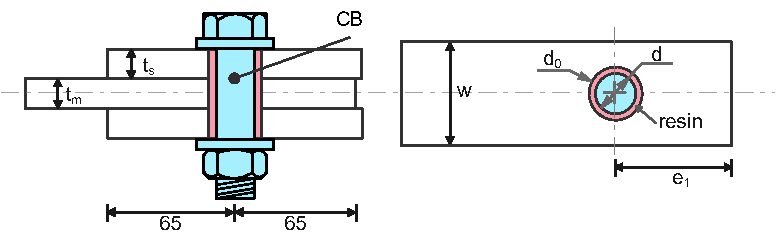
\includegraphics[width=0.8\textwidth]{imgs/app3/FEmodel-RIBJ.pdf}
    \caption{ Schematic illustration of FE model (unit: mm)}
    \label{fig-FEmodel-RIBJ}
\end{figure}

The analysis consists of three steps as shown in Table \ref{tab-app3-1}. The first step involves applying a pretension to the bolt by forced displacement (the relationship between forced displacement and pretension is obtained through prior calibration). The second step involves applying a displacement load (DL) of 0.01mm at the end of the main plate. The purpose of this step is to bring the pretension of the bolt into a stable state and to ensure firm contact between the bolt, resin, and bolt hole. The third step involves the application of the displacement load.


\begin{table}[htbp]
    \centering
    \caption{Analysis step} \label{tab-app3-1}
    \begin{tabular}{llll}
    \toprule
    FE Methods & Step-1 & Step-2 & Step-3 \\
    \midrule
    Execution Content & Apply Pretension & 0.01mm DL for stable & 3mm DL\\
    AMP time     & 2 & 0.1 & 5\\
    \bottomrule
    
    \end{tabular}
\end{table}

The shape of a mesh mostly depends on the geometry of the volumes. Within this model, simplifications are made as shown in Fig. \ref{fig-mesh-div-RIBJ}. For example, the bolt does not contain threads or radii. The same applies to the geometry of the nut. The elements applied in the model were three-dimensional--eight-node solid elements with a reduced integration (C3D8R). 

For the contact boundary condition, the surface-to-surface discretization method was used to avoid surface penetration, while the finite sliding tracking approach allowed for unrestricted movement of the contact surfaces. To simulate boundary nonlinearity, hard contact and penalty friction were employed to define the normal and tangential behaviours of the contact pairs, with isotropic Coulomb friction modelling the frictional forces.

The bolt head is fixed to the washer, and a slip coefficient of 0.4 is set for the faying surface between the main plate and the splice plate. For the resin-to-bolt hole and resin-to-bolt contact, see reference (15), a friction coefficient of 0.8 is set considering the viscosity of the resin.

\begin{figure}
    \centering
    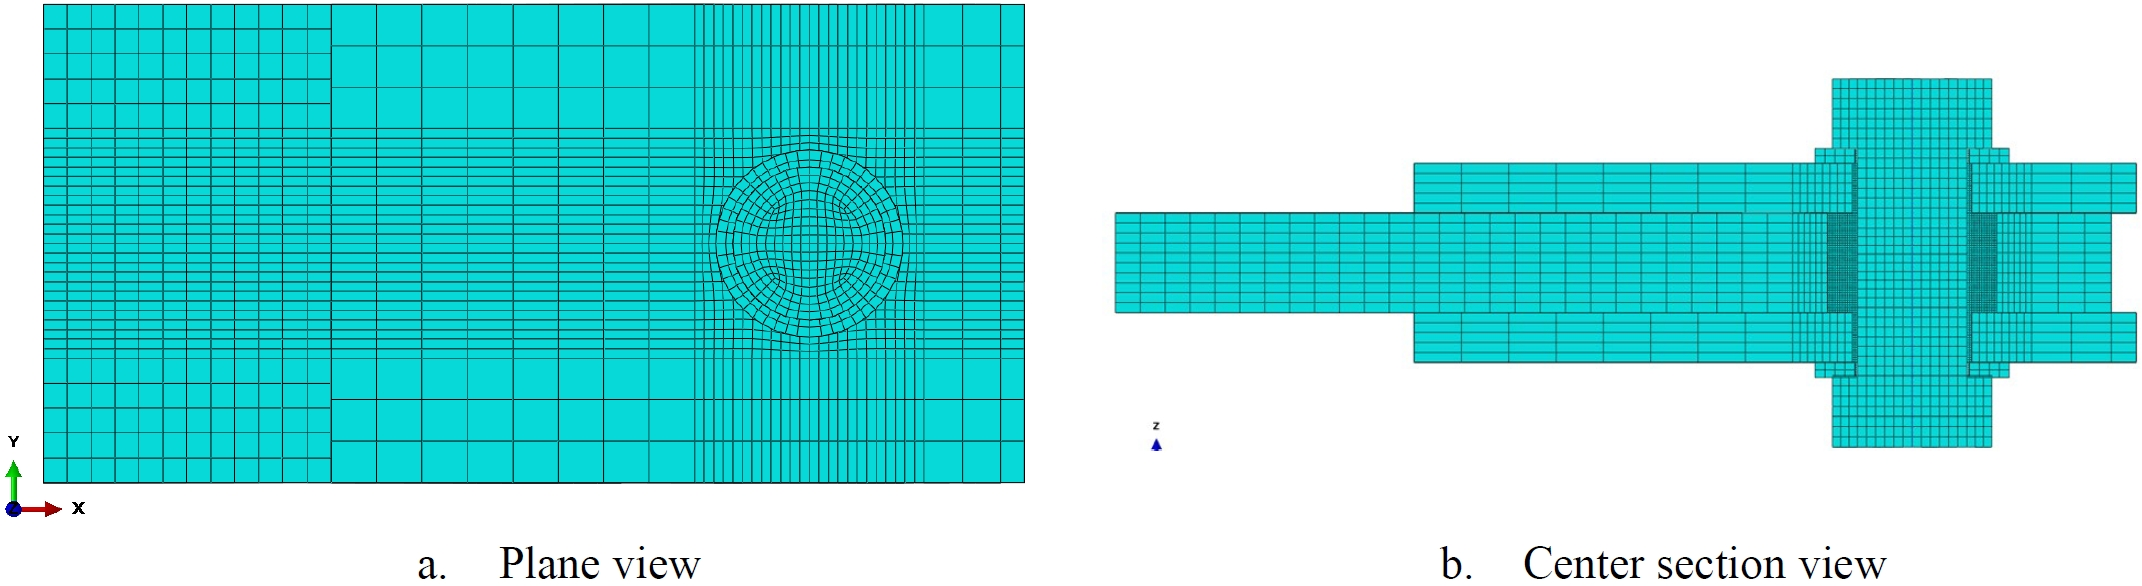
\includegraphics[width=0.85\textwidth]{imgs/app3/mesh-div-RIBJ.png}
    \caption{Mesh size and division of FE model}
    \label{fig-mesh-div-RIBJ}
\end{figure}

\subsection{Material properties}

This study primarily investigates three commonly used resin materials: Resin A (RenGel® SW 404 + Ren© HY 5159), Resin B (RenGel® SW 404 + Ren© HY 2404), and injection Steel-Reinforced Resin A (iSRR) which is Resin A filled with steel shots (SR-Res-A case). S355 steel was used for both the main and splice plate, and 10.9 grade bolts were used. The material properties are shown in Table \ref{tab-app3-2}.

\begin{table}[htbp]
    \centering
    \caption{Material properties}\label{tab-app3-2}
    \resizebox{\textwidth}{!}{
    \begin{tabular}{ccccc}
    \toprule
         & 
    \begin{tabular}[c]{c} Yong's Module $E$  \\ {[}Gpa{]} \end{tabular} &
    \begin{tabular}[c]{c} Poison ratio $v$  \\ {[}-{]} \end{tabular} &
    \begin{tabular}[c]{c} Yield strength $\sigma_y$  \\ {[}Mpa{]} \end{tabular} &
    \begin{tabular}[c]{c} Ultimate strength $\sigma_u$  \\ {[}Mpa{]} \end{tabular}\\
    \midrule
    Main \& Splice plate (S355) & 210 & 0.3 & 355 & 471 \\
    High Strength bolt (10.9) & 205 & 0.3& 900 & 1000 \\
    Resin-A & 11.7 & 0.3 & 125 & - \\
    Resin-B & 5.7 & 0.3 & 140 & - \\
    SR-Res-A & 30 & 0.3 & 135 & - \\
    \bottomrule
    \end{tabular}
    }
\end{table}

The FEA in this study employs the Drucker-Prager model for resin. The properties of the resin are obtained from the available literature (6, 12, 15), and the specific parameters used are detailed in Table \ref{tab-app3-3}. Additionally, the hardening characteristics of the resin are considered, as indicated in Table A1. The values mentioned above pertain to the associated and unconfined properties of the resin. The associated parameters are assumed due to their significantly lower chance of divergence. On the other hand, the unconfined properties are chosen as implementing confined conditions is expected to overestimate the resin's behaviour. 


\begin{table}
    \centering
    \caption{Material Parameters of the linear Drucker-Prager model (Associated flow)}
    \label{tab-app3-3}
    \begin{tabular}{lccc}
    \toprule
    Name & $\beta$ [$^{\circ}$] & $\kappa$ [-] & $\psi$ [$^\circ$] \\
    \midrule
    \begin{tabular}{l} Res-A \cite{pedrosa2022injbolt-mec}  \\ (RenGel® SW 404 + Ren© HY 5159) \end{tabular} &
    35.42 & 0.778 & 35.42\\
    \begin{tabular}{l} Res-B \cite{xin_computational_2019}  \\ (RenGel® SW 404 + Ren© HY 2404) \end{tabular} &
    10.33 & 0.93 & 10.33 \\
    \begin{tabular}{l} SR-Res-A (iSRR) \cite{pedrosa2022injbolt-mec}   \\ (Res-A + Steel shots) \end{tabular} &
    54.28 & 0.778 & 54.28 \\
    \bottomrule
    \end{tabular}
\end{table}

\subsection{Analysis case}

Table \ref{tab-app3-4} illustrates the analyzed cases, which explore the load transmission mechanism of the pretension injection bolted connection based on the resin type and the oversized hole.

\begin{table}[htbp]
    \centering
    \caption{Analysis case (Unite: mm)}
    \label{tab-app3-4}
    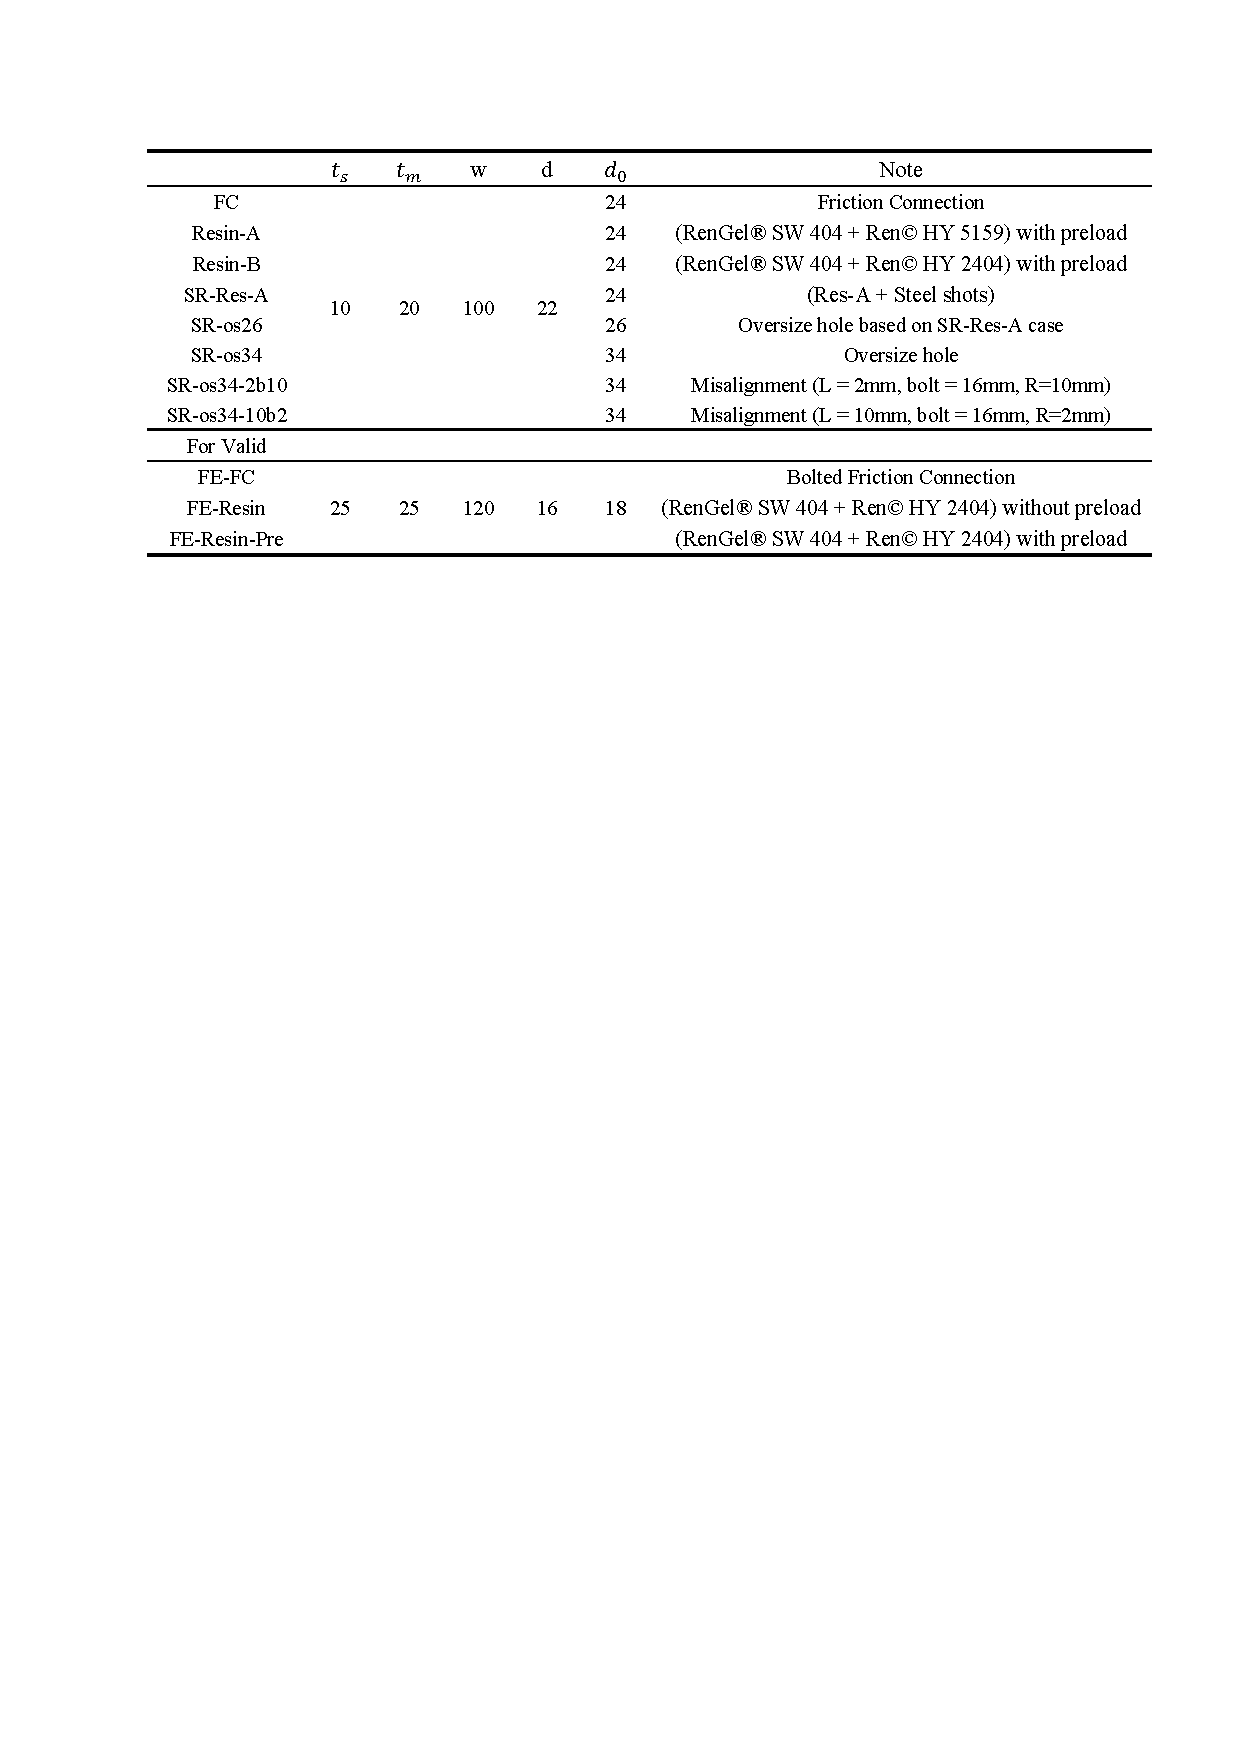
\includegraphics[width=\textwidth]{imgs/app3/ana-case-RIBJ.pdf}
    
\end{table}

\subsection{Validation of FE analysis}

\begin{figure}[htbp]
    \centering
    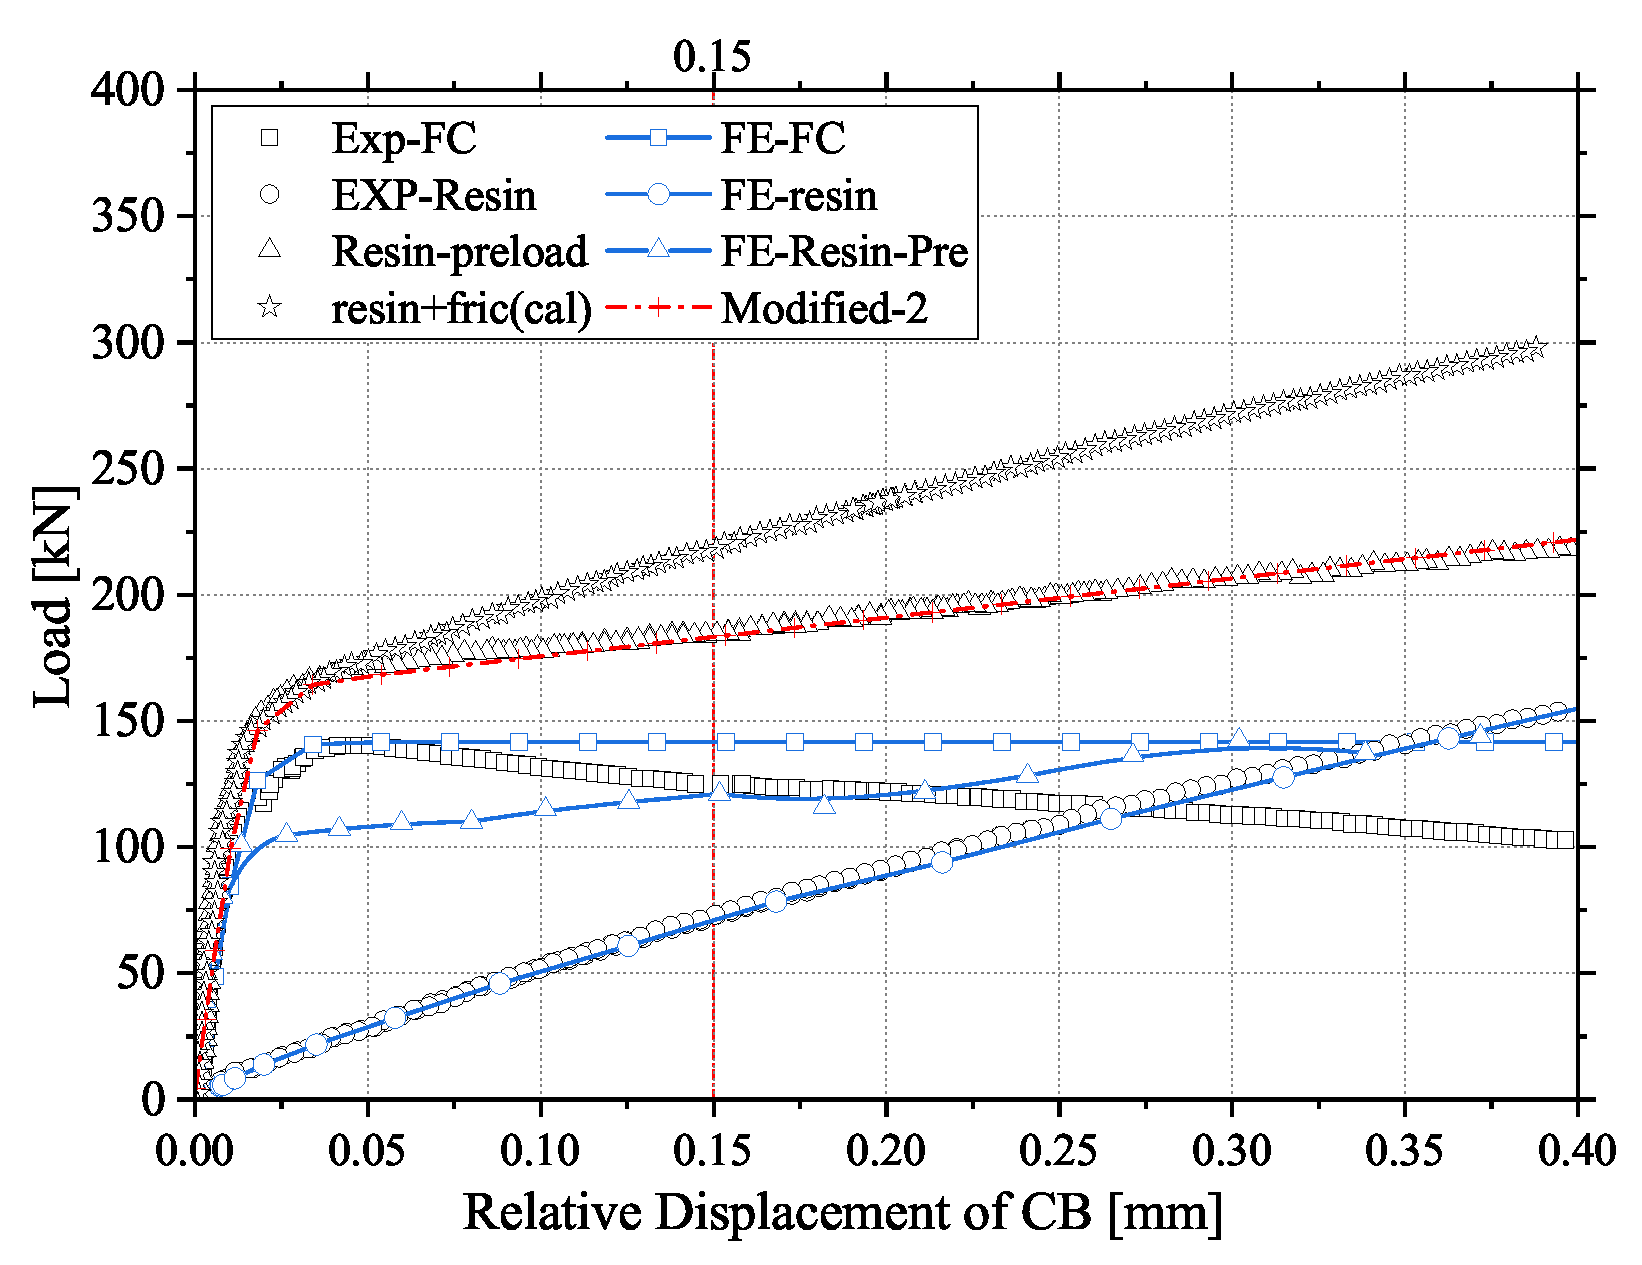
\includegraphics[width=0.65\textwidth]{imgs/app3/valid-RIBJ.eps}
    \caption{Compare between experiment results \cite{derks_msc_2023} and analysis results.}
    \label{fig-valid-RIBJ}
\end{figure}

Fig. \ref{fig-valid-RIBJ} illustrates the experimental and analytical results for a double-lap single bolted connection. The black plot represents the experimental results, while the solid blue line represents the analytical results. The following legend is used:

\begin{table*}[h]
    \centering
    \begin{tabular}{ll}
     FC:&  represents the friction connection with clearance between the bolt and hole;  \\
     Resin: & represents the Resin-B injection bolted connection without preload; \\
     Res+pre: & represents the resin-B injection bolted connection with preload applied.
    \end{tabular}
\end{table*}
 
Additionally, the “resin+fric(calc)”   curve with the start symbol represents the load-displacement curve obtained by adding the resistance of the friction connection and the injection bolted connection (in other words, this curve represents the resistance calculation method of Eurocode3. The bearing strength of the Resin-B can be calculated as 162 MPa by referencing EN 1090-2:2018 Annex J with the formula $f_{(b,resin)}=F_{0.15}/A_s$.

From, for the “Resin-Pre” case, the analytical results are almost identical to the experimental results. For the friction connection, the analytical results exhibit the same behaviour as the experimental results before the slip occurs. However, since the analysis utilises the Coulomb friction model and does not consider the decay, the friction coefficient will not change after reaching the slip resistance, and it will still be proportional to the contact pressure.

\section{Results and Discussion}

\subsection{Relative Displacement}

\begin{figure}[htbp]
    \centering
    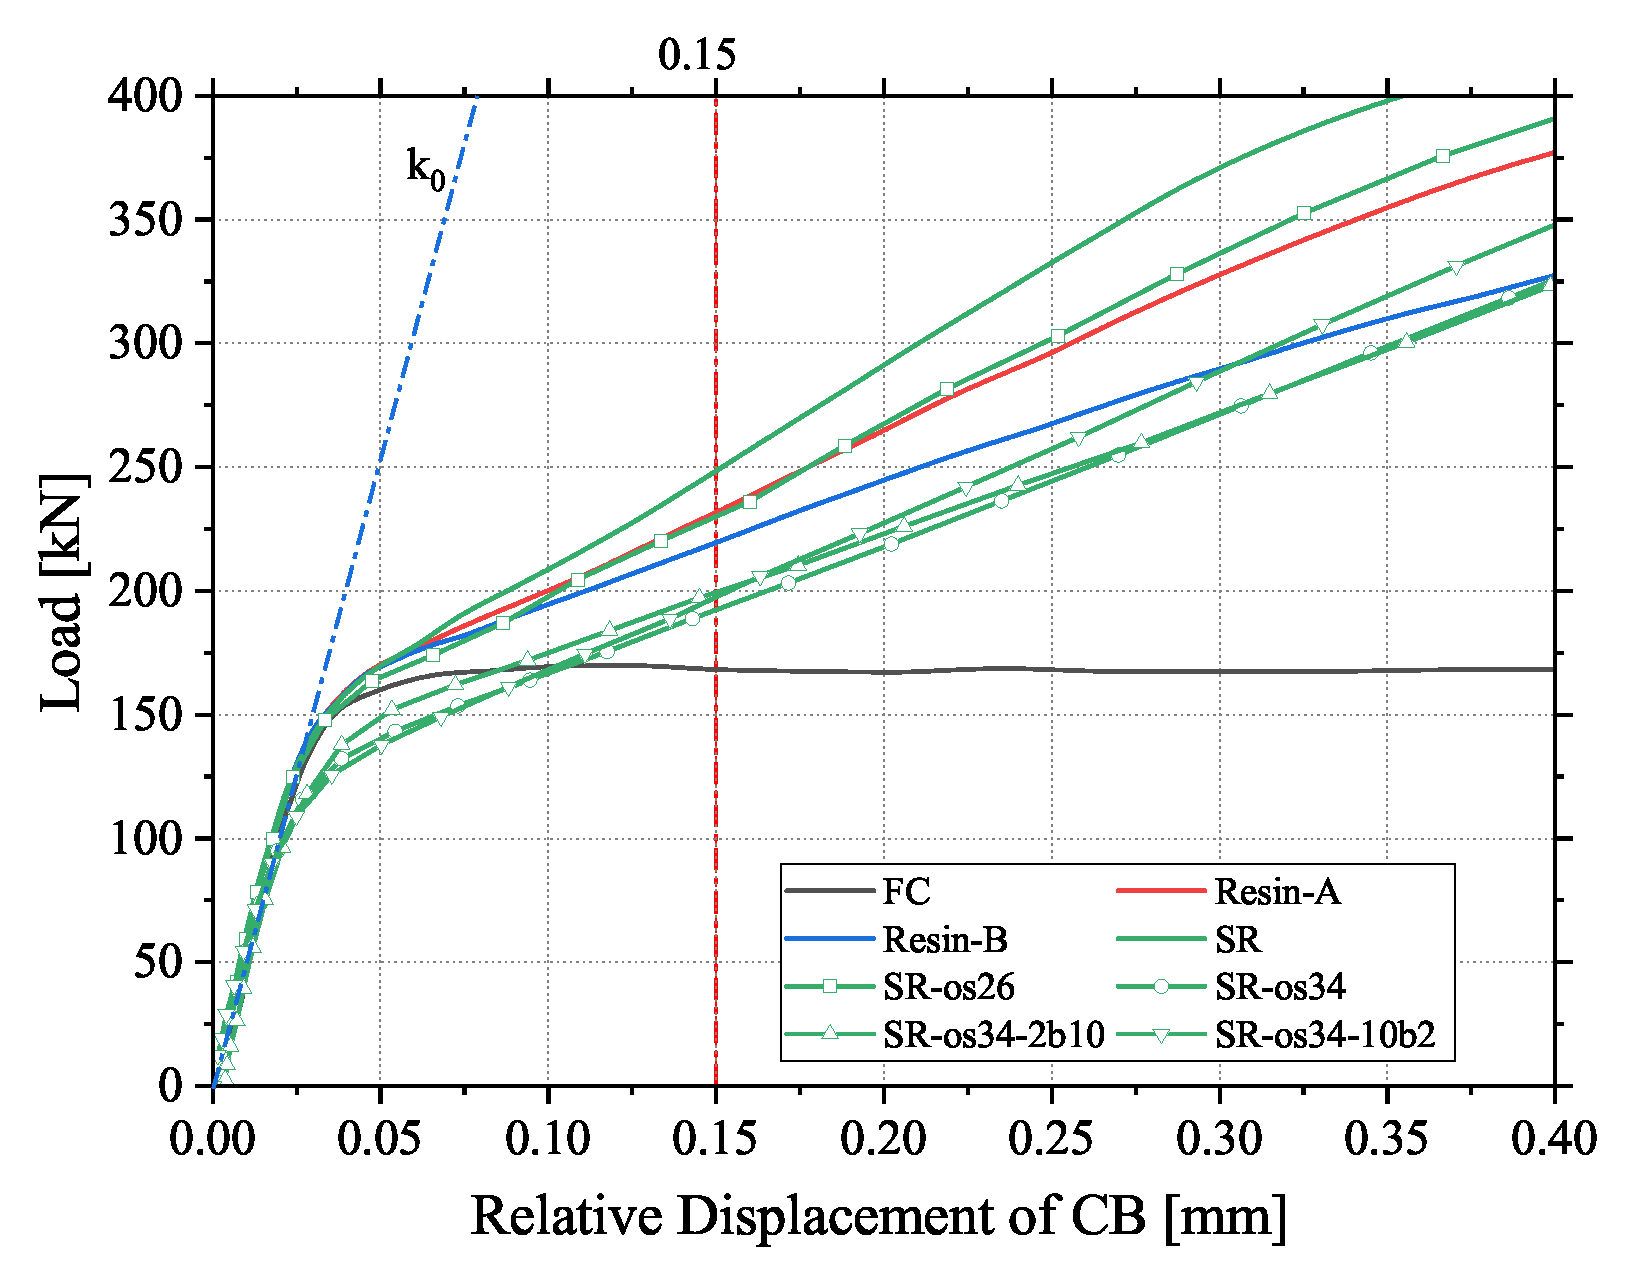
\includegraphics[width=0.65\textwidth]{imgs/app3/RD-RIBJ.eps}
    \caption{The relationship between load and Relative Displacement of CB position}
    \label{fig-RD-RIBJ}
\end{figure}

Fig. \ref{fig-RD-RIBJ} shows the relationship between the load and relative displacement of the analysis result. It can be observed that regardless of using different resins or using oversized holes, the initial stiffness $k_0$ of the injection bolted connection hardly changes. In the case of load transmission through friction and bearing, the friction provides higher stiffness and primarily transmits most of the load. Therefore, the initial stiffness of the injection bolted connection is mainly determined by the friction contribution, as confirmed by a previous study \cite{Chen2023MechanicalConnections}. Additionally, it can be observed that in the second slope, the slopes of SR-Res-A, Resin-A, and Resin-B decrease sequentially. This decrease is almost proportional to Young’s modulus, which indicates that the stiffness of the joint, after surpassing the slip resistance, is primarily determined by the bearing resistance.

For the oversized hole cases, it can be observed that as the bolt hole size increases, the point of change in initial stiffness decreases. When the bolt hole size reaches 34mm, the point of change in initial stiffness has significantly decreased. This can be attributed to the tendency of the splice plate to deform easier as the bolt hole size increases, resulting in a decrease in friction force.
For the case of “misaligned bolt position”, it can be observed that the point of change in initial stiffness is higher for 2b10 with 2mm clearance of tensile side, while it is lower for 10b2 with 10mm clearance  . This is because the size of the clearance on the tensile side determines the ease of deformation of the splice plate, thereby altering the friction force. In contrast, the second slope of 2b10 with 10mm clearance of the compressive side is lower compared to 10b2 with 2mm clearance. This is because a thicker resin makes deformation more likely to occur, decreasing the second slope determined by the bearing connection.

\subsection{Load sharing of bearing and friction}

\begin{figure}[htbp]
    \centering
    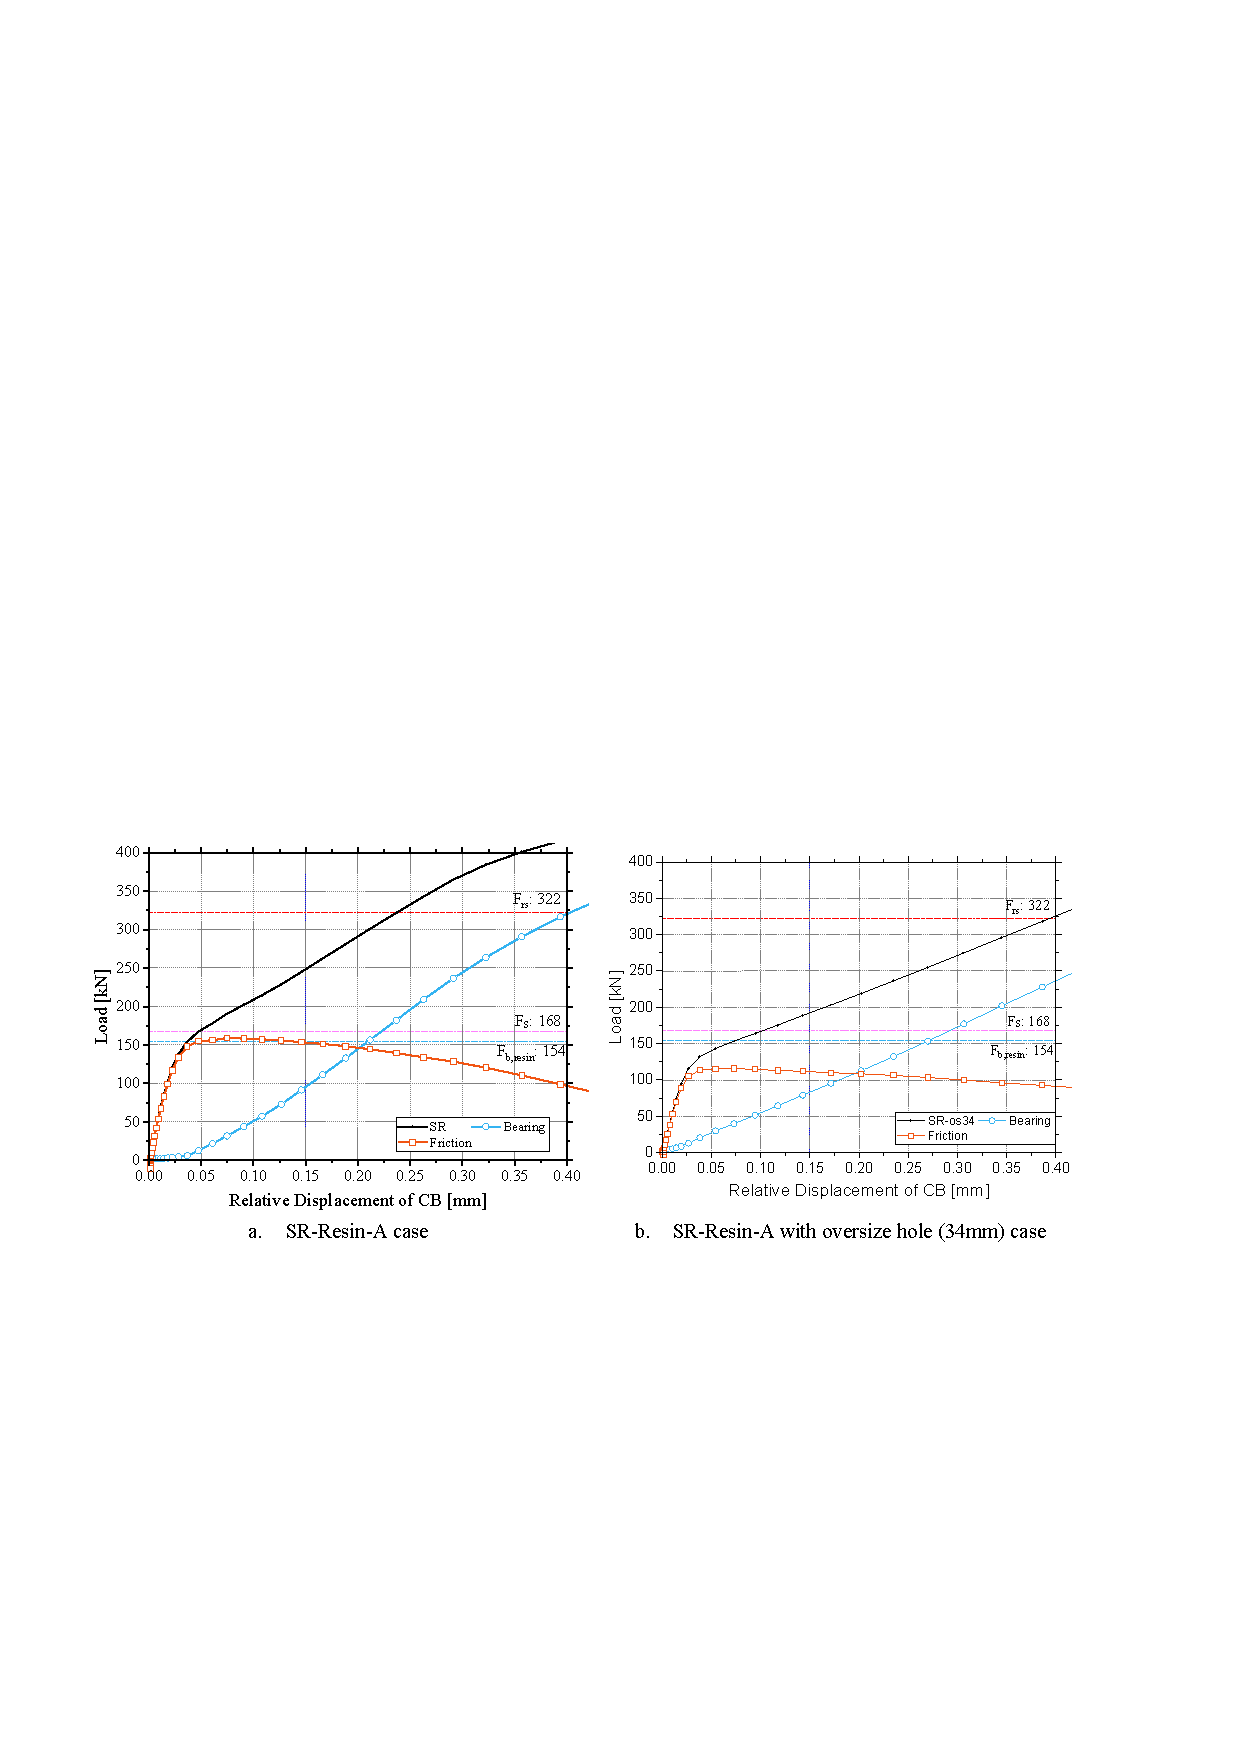
\includegraphics[width=\textwidth]{imgs/app3/LDS-RIBJ.pdf}
    \caption{Load sharing of bearing and friction force.}
    \label{fig-LDS-RIBJ}
\end{figure}

Fig. \ref{fig-LDS-RIBJ} shows the load sharing between bearing and friction contribution for SR-Resin-A and SR-Resin-A with 32mm oversize hole case. where the friction force is the total force calculated by the shear stress of the top surface in the main plate, the bearing force is the total force calculated by the sum of the contact pressure of the hole surface, and the tensile force is the end of main plate total section force.

The resistance of iSSR connection $F_{rs}$ is calculated by Eq.\ref{eq-app3-1}, where $f_{(b,resin)}$ is 351 MPa based on the research of Nijgh \cite{nijgh_new_2017}. Eurocode 3 provides reduction factor $k_s$ for oversized holes in terms of slip resistance for friction connections and bearing resistance for injection bolt connections without considering pretension. However, for a pretension injection bolt, it is necessary to consider the interaction between friction and bearing. To discuss the load reduction rate for pretension injection bolt force and oversize holes clearly, the reduction factor $k_s$ are not separately considered in the resistance calculation.

\begin{equation}\label{eq-app3-1}
    F_rs=F_s+F_{(b,Rd,resin)}
\end{equation}

\begin{equation}
    F_s=μmN
\end{equation}

\begin{equation}
 F_{(b,Rd,resin)}=dt_m f_{(b,resin)}
\end{equation}

Where the $μ$ is the friction coefficient, m is the number of friction plane,  $N$ is the bolt pretension, $d$ is the diameter of the bolt, $t_m$ is the thickness of the main plate.

In Fig. 6.a, it can be observed that before the resin starts transmitting load by bearing, the joint primarily transfers load through friction. Since the analysis employs the Coulomb friction model, the friction coefficient remains unchanged. Therefore, the decrease in friction force can be attributed to the bearing, which will be explained in the next section regarding the mechanism of friction force reduction. Thus, it can be concluded that without considering the decay of kinetic friction, the decrease in friction force due to bearing is 0.89 at a relative displacement of 0.15mm.

During the initial stages, the load transmission in the joint is primarily achieved through friction. As a result, the resin-based bearing connection is unable to maintain its initial stiffness. When the friction contribution is approaching its maximum slip resistance, the load transmission in the bearing becomes fully effective. This stage can be referred to as the friction / bearing hybrid load transmission stage. Therefore, when the relative displacement reaches 0.15, the bearing connection cannot achieve its original bearing load without pretension (which is 154 kN). For the SR-Resin-A case at 0.15 mm, the load decreases to 97 kN (reduction rate of 0.63).

As shown in Fig. 6.b. the SR-os34 case also exhibits a similar trend with SR-Resin-A case, though the decrease in friction force is significantly more pronounced compared to the standard hole case (reduced to 111 kN, with a reduction rate of 0.66). Furthermore, it has been found that for the oversize hole, the secondary slope (i.e., bearing stiffness) of the bearing connection is lower than that of the standard hole. This can be attributed to the fact that the resin with a lower elastic modulus occupies a larger area, making the joint more susceptible to deformation and resulting in lower stiffness.

\subsection{Reduction of friction force due to friction and bearing interaction}

The cross-sectional force acting on the main plate is divided into the cross-sectional forces of the main plate and splice plates via the shear transmit on the bolt. Assuming that the point of action of each cross-sectional force is at the centre of the plate, an additional bending moment is generated in the bolt due to the eccentricity of the cross-sectional forces. The boundary condition at the end of the connection plate is free, so there is a tendency to deform outward toward the main plate faying surface when subjected to additional bending moments, resulting in a separation of the connection plate from the main plate, and therefore a loss of friction force.

Fig. \ref{fig-u3cmap-ribj} shows the deformation contour plot of the joint in the U3 (z) direction, where it is evident that the splice plate undergoes deformation due to the additional bending moment generated. Additionally, the oversize hole has a larger clearance, and even with resin injection, the splice plate is still prone to deformation due to the resin's lower stiffness.

In the compressed side of bolt where the bolt generates additional bending moment, due to bolt deformation, higher contact pressure is generated at the compressed side, as observed in Fig. \ref{fig-pressmap-ribj}-b. However, there is an overall decreasing trend in the total contact pressure of faying surface.

\begin{figure}[htbp]
    \centering
    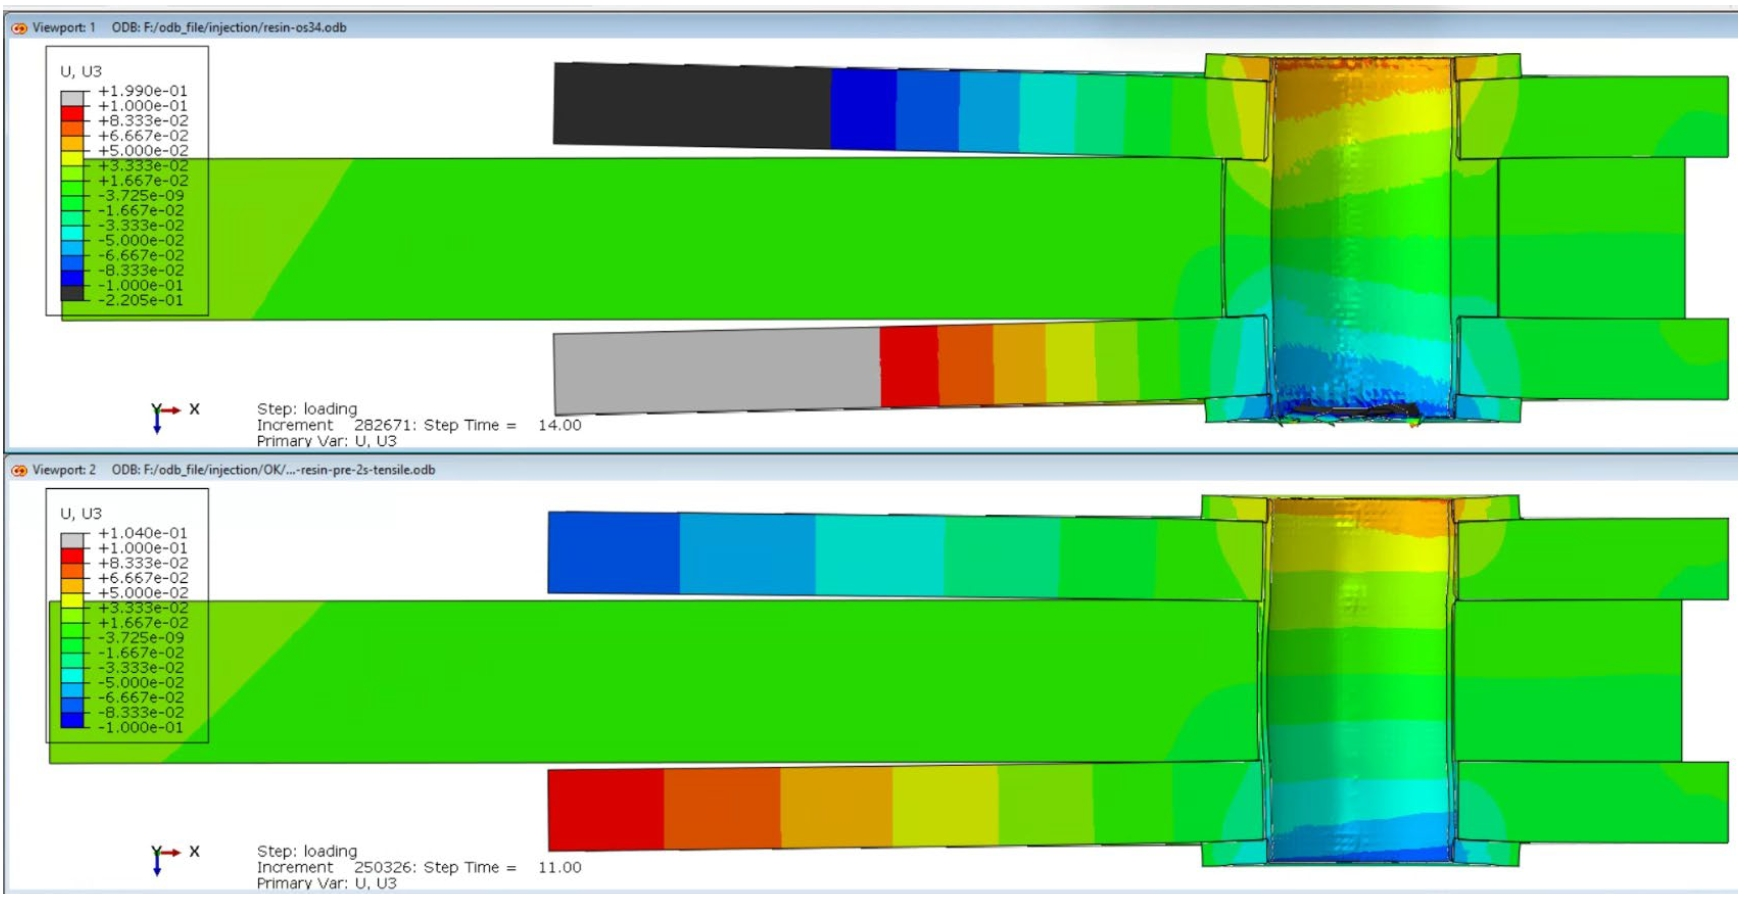
\includegraphics[width=0.9\textwidth]{imgs/app3/U3Cmap-RIBJ.png}
    \caption{ The counter map of U3 (z) direction deformation when the relative displacement is 0.15mm. The above one is SR-os34, lower one is SR-Res-A case (deformation scale: 1.0).}
    \label{fig-u3cmap-ribj}
\end{figure}


\begin{figure}[htbp]
    \centering
    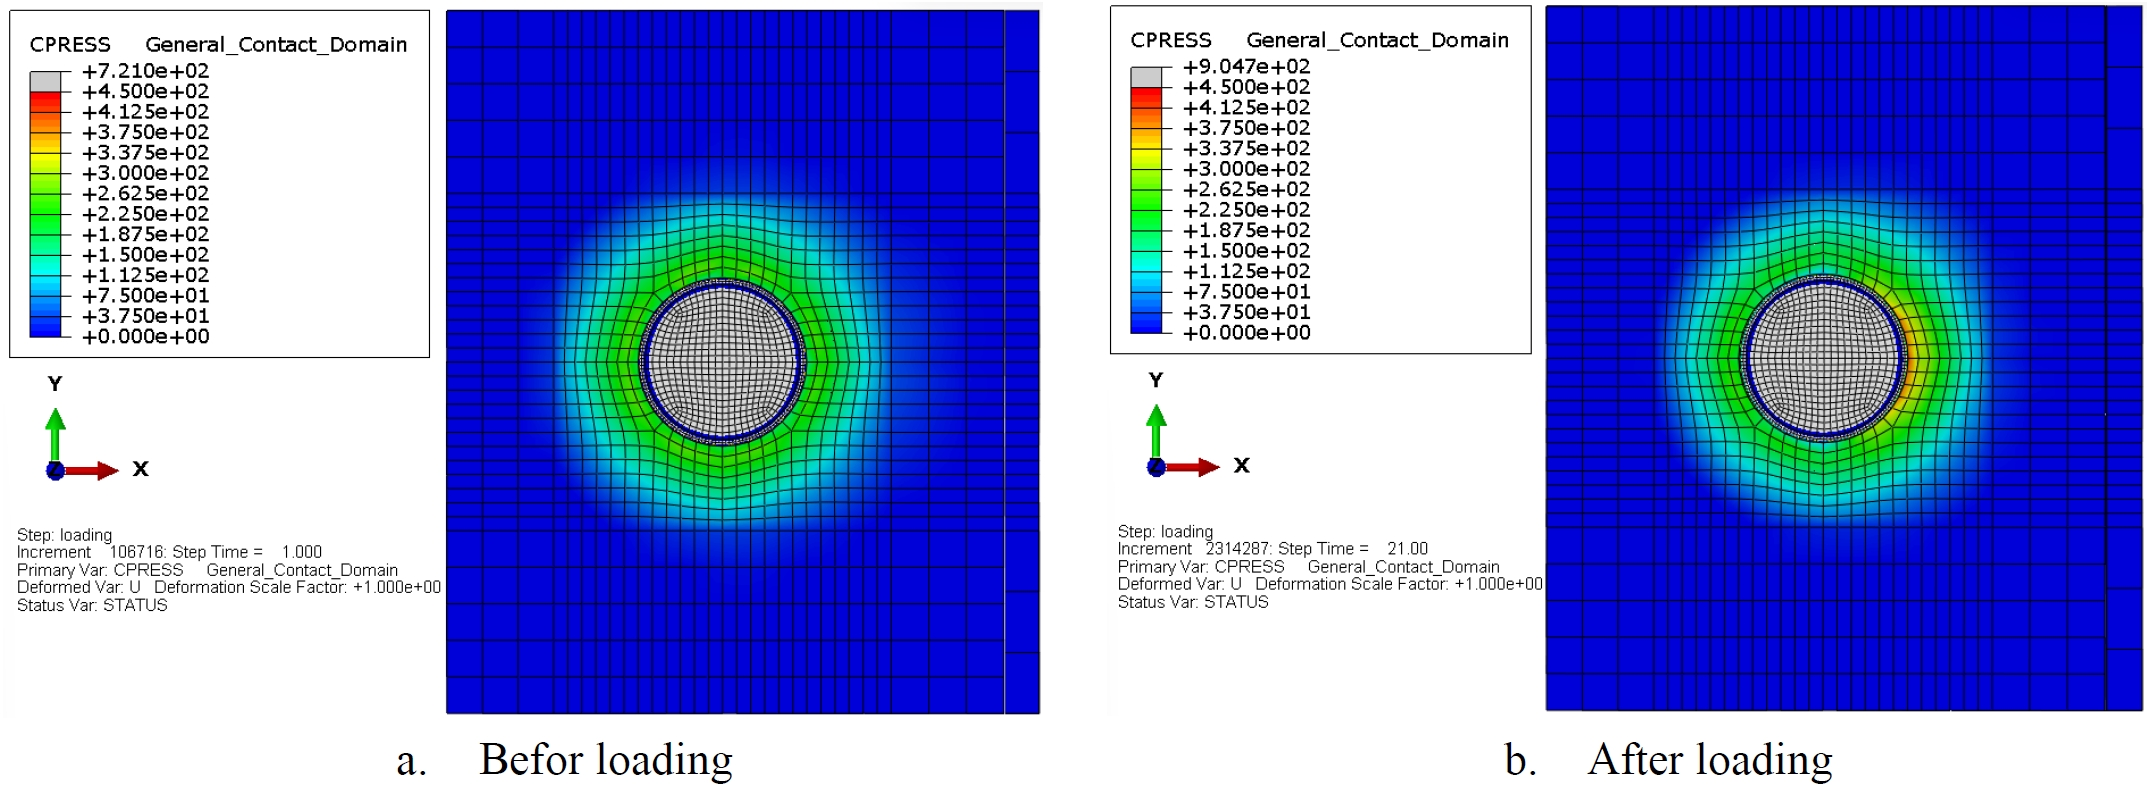
\includegraphics[width=0.9\textwidth]{imgs/app3/pressmap-RIBJ.png}
    \caption{The contact pressure contour map of SR-Res-A case}
    \label{fig-pressmap-ribj}
\end{figure}

\subsection{Discussion the slip resistance of pretension injection bolted joint}

\begin{table}[htbp]
    \centering
    \caption{The reduction rate of pretension injection bolted connection.}
    \label{tab-app3-5}
    \begin{tabular}{cccccc}
    \toprule
    \begin{tabular}{c} Reduction \\ rate \end{tabular} & SR-Res-A & SR-os26 &SR-os34 &Resin-B &
    \begin{tabular}{c} Dieter’s experiment \\ (Resin-B) \cite{ungermann2023injbolt-mec} \end{tabular} \\
    \midrule
    Friction & 0.89 & 0.87 & 0.66 & 0.94 & - \\
    Bearing & 0.63 & 0.56 &  0.53 & 0.81 & - \\
    Total & 0.77 & 0.72 & 0.60 & 0.88 & 0.85 \\
    \bottomrule
    \end{tabular}
\end{table}

Table \ref{tab-app3-5}. summarizes the reduction rate of load in the pretension injection bolted connection. Different resin types and the case of oversized holes are compared. It can be observed that the load reduction rate is significant for the SR-Resin-A, especially for the bearing force, reaching a reduction rate of 0.77. The reduction rate in friction force is 0.89, encase a lack of consideration for dynamic friction, so the actual reduction rate is expected to be lower than this value. Comparison with Dieter's experimental data (7) reveals that for the same type of Resin-B case, the analytical reduction rate (0.88) is higher than the experimental value (0.80), possibly due to the omission of dynamic friction in the analysis. Additionally, as the hole size increases, the reduction in friction force decreases significantly from 0.89 to 0.66, while the bearing force only decreases from 0.63 to 0.53. Therefore, it can be concluded that friction force is more sensitive to hole enlargement.

The current design formula in Eurocode3 simply adds the bearing force and friction force, which is unreasonable and needs to consider the interaction between friction and bearing. Moreover, the calculation of the reduction rate largely depends on how the bearing strength is obtained. Due to the lack of experiments on iSSR bolted connections, the bearing strength of the SR-resin-A used in this analysis may be overestimated. Obtaining the correct bearing strength of the resin is also an issue of consideration.

\section{Summarize and Further research}

\subsection{Summarize}

This work investigated the load transmission mechanism and examined the interaction behaviour between the frictional resistance $F_{(s,Rd)}$ and the bearing resistance $F_{(b,Rd,resin)}$ of injection bolted connections with pretension by comparing bearing / friction and hybrid (bearing + friction) connection, resin types and oversized holes and analysing experimental data. Based on the results of our investigation, we have made the following findings and conclusions.

\begin{enumerate}
    \item The load is initially transmitted through the higher rigidity friction resistance for injection bolted connections with pretension force. The bearing resistance is gradually activated when the friction resistance approaches its maximum (slip resistance).
    
    \item In the analysis without considering dynamic friction decay, the friction force decreases. This is because when the bolt is subjected to shear, the additional bending moment leads to out-of-plane deformation of the splice plate, reducing contact pressure. 
    
    \item The reduction in friction force is particularly significant with the oversized hole. Additionally, enlarging the hole means that more resin is needed, making the joint more susceptible to deformation and decreasing the bearing connection's stiffness.

    \item For an oversized hole, the misalignment of the bolt does not significantly alter the load transfer behaviour of the connection. When there is more resin on the tension side and less resin on the compression side (SR-os34-10b2), there will be a greater reduction in friction force and a higher stiffness in the bearing connection, and vice versa.
    
    \item The slip resistance of pretension injection bolted joint cannot be obtained simply by adding friction resistance of individual bolt $F_s$ and bearing resistance of resin $F_{(b,resin)}$ and needs to consider the interaction between friction and bearing.

    
\end{enumerate}

\subsection{Further research about the RIBJ}

Next, a parametric study will be conducted on the geometric shape of the connection based on FEA (such as enlarged hole, plate thickness) to quantify the interaction between friction and compression. Then, a strength correction factor considering the mixed interaction of the connection will be proposed.

For injection steel-reinforced resin (iSRR) bolted connections with pretension, there is a lack of experimental data, and further experiments are needed to obtain reliable bearing strength. 


\section{Drucker Prager Hardening}

The data of the Drucker prager hardening  law in the analysis are shown in the Table \ref{tab-DPH-data}.

\begin{table}[htbp]
    \centering
    \caption{The Model of Drucker Prager Hardening}\label{tab-DPH-data}
    \begin{tabular}{llllll}
    \toprule
\multicolumn{2}{c}{Res-A} & \multicolumn{2}{c}{Res-B} & \multicolumn{2}{c}{SR-Res-A} \\
 
\begin{tabular}{l} True \\ stress\end{tabular} &
\begin{tabular}{l} True \\ plastic strain\end{tabular} &
\begin{tabular}{l} True \\ stress\end{tabular} &
\begin{tabular}{l} True \\ plastic strain\end{tabular} &
\begin{tabular}{l} True \\ stress\end{tabular} &
\begin{tabular}{l} True \\ plastic strain\end{tabular}  \\
\midrule
	125.0	&0	&80	&0	&135.0	&0 \\
	120.0	&0.0115	&85	&0.0012	&136.2	&0.0039 \\
	115.0	&0.0395	&90	&0.00258	&130.0	&0.0074 \\
	110.0	&0.0895	&95	&0.00410	&100.0	&0.0154 \\
	106.0	&0.1895	&100	&0.00571	&20.0	&0.0354 \\
			&105	&0.00774 &		& & \\
			&110	&0.01023 &		& & \\ 
			&115	&0.01338 &		& & \\
			&120	&0.01859 &		& & \\ 
			&125	&0.03513 &		& & \\
			&130	&0.07320 &		& & \\
			&135	&0.10626 &		& & \\ 
			&140	&0.15648 &		& & \\
 \bottomrule
    \end{tabular}
\end{table}